% Activate the following line by filling in the right side. If for example the name of the root file is Main.tex, write
% "...root = Main.tex" if the chapter file is in the same directory, and "...root = ../Main.tex" if the chapter is in a subdirectory.
 
%!TEX root =  ../A Survey of 3D Algorithm

\chapter[Preface]{A Narrow Introduction to 3D world}
% 这是开始尝试用程序员的方式写工作记录的第一天。2023-11-06
人眼采集视觉信息对物体进行描述,可以从颜色/亮度/大小/等不同维度展开,这些因素会被相机以怎样的方式采集和呈现呢?\par
当人获取2D/3D相机的信息后,又需要以怎样的方式对像素数据加以处理,才能获得人能理解和接受的数据呢?
要解答这些问题,就必须要理解3D信息是怎样被照相机获取的,Depth相机相较于常规的RGB相机,又增添了怎样的处理流程?从3D高维数据降低到2D维度时,哪些信息会有丢失或损毁?\par
为了回答这些问题,就需要对相机成像的过程进行深入了解,知道相机内参/外参/畸变参数的物理含义,知道相机畸变校正/极线校正的基本过程,了解2D图像和空间点云的对应关系。这些内容,在后续这些章节中,会逐一展开详细叙述。

\section{Introduction}
本章节,将从几何光学的角度对基础内容进行介绍。在单目几何中,依托小孔成像过程,介绍齐次坐标,相机内参,畸变参数,外参等基础概念。\par
在双目几何中,待介绍的内容待定。\par
在对极几何中,会重点介绍对极点,对极线,基础矩阵,本质矩阵等概念。\par
在相机标定中,会综合运用前述章节的知识,以相机的标定过程为例,展示前述知识的实际应用。
\section{Single View Geometry}
在小孔成像过程中,常见的过程可以表示如下:
\begin{figure}[H]
\centering
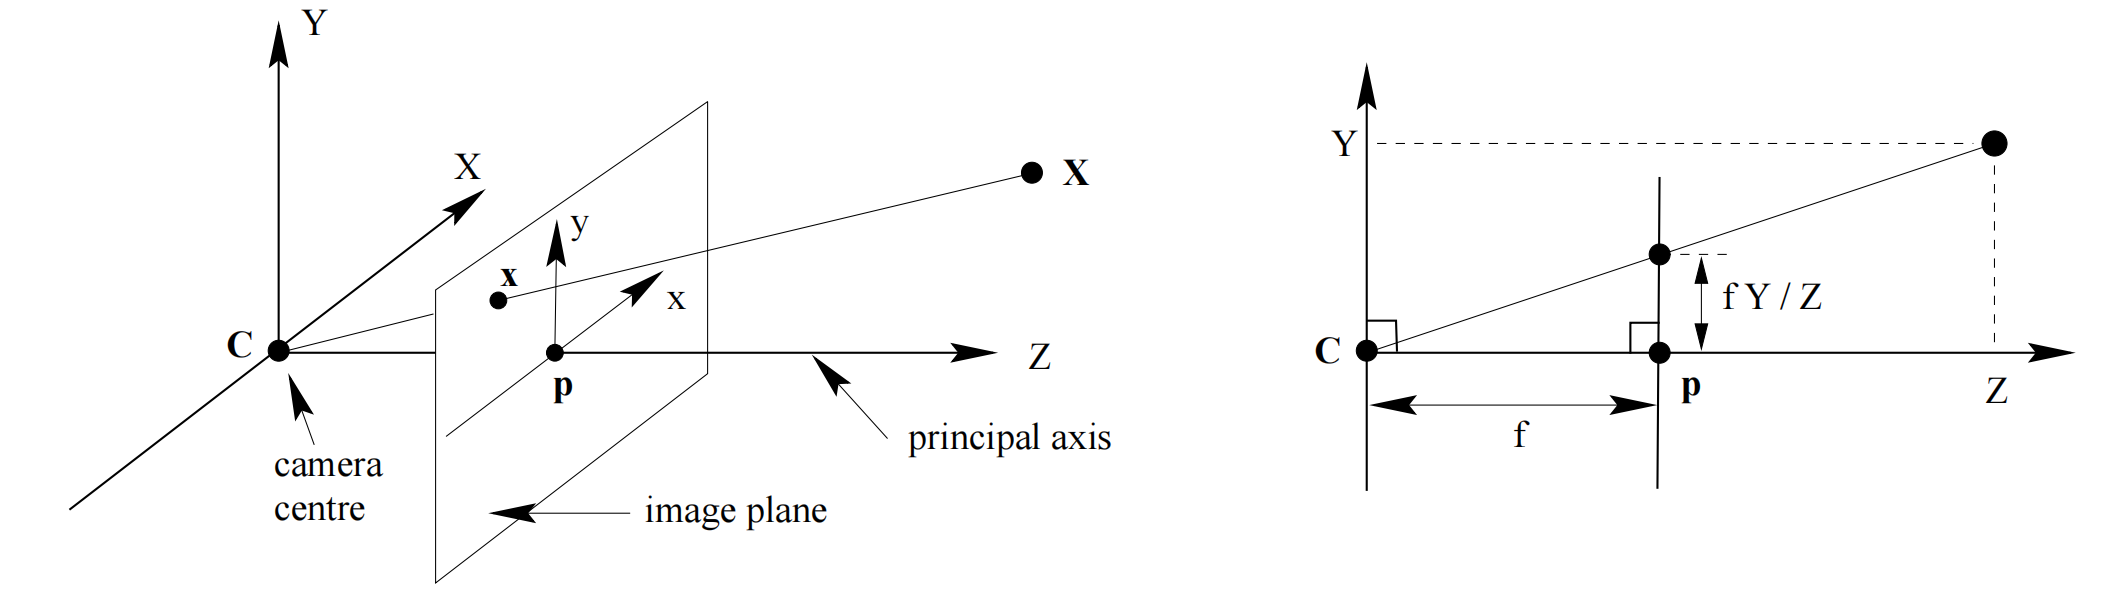
\includegraphics[scale=0.3]{Chapter1/PinholeCameraModel.png}
\caption{Pinhole Camere Model}
\end{figure}
在世界坐标系下空间点\[X_w=[x,y,z]\]
从世界坐标系转化到Camera坐标系下为 \[X_c = RX_w+T\]
其中$R = R_cw$,代表从世界坐标系转化到Camera坐标系。\par
相机内参为
\[ K = \left[ \begin{array}{ccc} fx & 0 & cx \\ 0 & fy & cy  \\ 0 & 0 & 1 \end{array}\right] \]
投影到sensor上的像素坐标表示为\[\begin{array}{cc}u=x/z*fx+cx \\  v = y/z*fx+cy\end{array}\]
在通常的分析中,为了矩阵表达的简洁,采用齐次坐标的形式表达上述投影过程:
\[ \left[\begin{array}{ccc} u\\v\\1\end{array}\right]
=
K \left[ \begin{array}{c|c} R & T \end{array}\right] P_w
=
\left[ \begin{array}{cccc} fx & 0 & cx & 0 \\ 0 & fy & cy & 0 \\ 0 &  0 &  1 & 1\end{array}\right]
\left[ \begin{array}{cc} R & T\\0 &1 \end{array}\right]
\left[ \begin{array}{c} x/z \\y/z\\1\\1\end{array} \right]
\]
可以看到,在3维空间点投影到2维图像的过程中,Z的维度信息在在Sensor中是丢失的,即:3维空间中的点,投影到sensor上是明确的一个像素位置;但是sensor上的1个像素,对应到3D空间中
时,不能明确定义出一个点,只能定义出一条直线。为了更清晰地说明这个过程,我们可以写出从2D像素点逆投影到3D空间的过程如下:
\[
\begin{array}{ccc} x&=& P_{proj}X_c \\ X_c^{length less} & = &P_{proj}^\dagger x \end{array}
\]
其中,$P_{proj}^\dagger$ 是投影矩阵$K \left[ \begin{array}{c|c} R & T \end{array}\right] $的广义逆,得到的只能是$\left[ \begin{array}{c} x/z \\y/z\\1\\1\end{array} \right]$形式的沿Z轴归一化的一个结果,即为空间中的一条射线。
这条射线已知穿过空间中的2个点:sensor对应的光心$C$和该像素点$[u , v]$,根据这两个点,即可得到空间中射线的坐标。假定已知光心为$C=[x_c, y_c, z_c]$,sensor像素坐标下下某点为$x=[u ,v, 1]$,首先将光心坐标转化为它在sensor坐标系下的坐标$C = [c_x, c_y , 1]$,这两个点都在$x$做逆向投影到3D空间形成的射线上。这条直线,在后续分析对极几何相关内容时,会有较大的用处。
\section{Epipolar Geometry}
对极几何,这个问题有一个非常典型的场景:对应同一个物体,用人的左右眼分别去看,会发现物体在“跳动”,物体和人眼的距离越近,这种“跳动”就越发显著。从相机成像的角度来看,我们不妨假设这样一个场景:使用同一台相机,在两个不同的位置拍摄同一个物体,拍摄出来的图片,会有怎样的特征?这个问题的答案,就在本节中。
\begin{figure}[H]
\centering
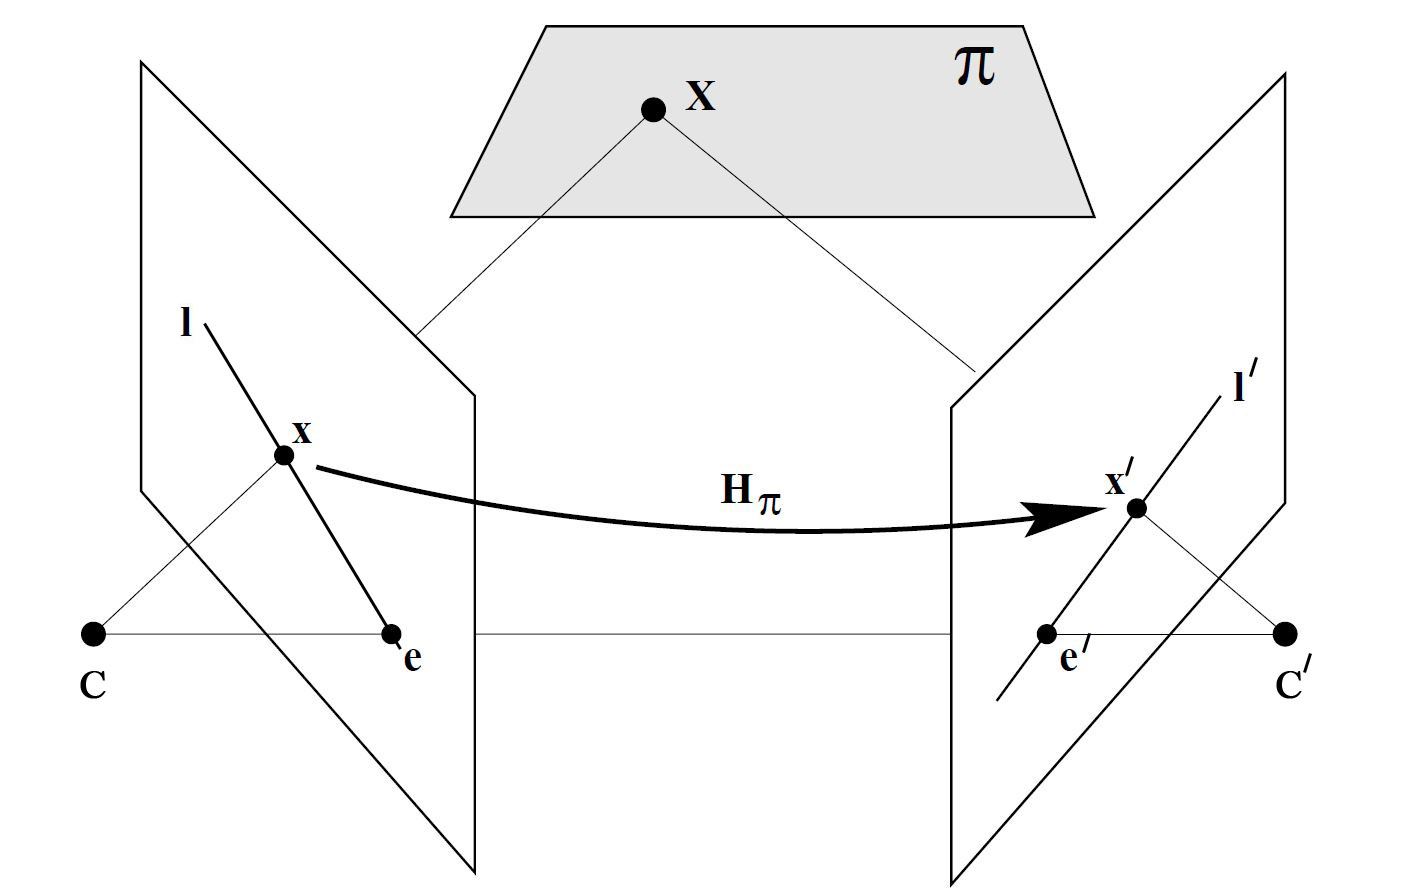
\includegraphics[scale=0.3]{Chapter1/DescriptionOfEpio.jpeg}
\caption{Description of Epipolar Geometry}
\end{figure}
在图中,内参相同的两个相机,光心分别为$C$和$C'$。它们同时对空间点$X$成像,对应在像素上的位置分别为$x$和$x'$。$C$h和$C'$的连线与各自sensor平面的交线为$e$和$e'$。在暂时忽略相机畸变的情形下,根据“光沿直线传播”的假设下,根据几何知识,不难推导出以下结论:
\begin{enumerate}
\item $e$和$e'$是两个相机在彼此眼中的位置,这两个点也被称作“对极点”;
\item $line C-->X$即为$x$逆投影到空间中时对应的射线,它在相机$C'$中对应与$line e' --> x'$;同样地,$line C' --> X$在$C$中成像为 $line e-->x$。 这两条线,被称为“对极线”;
\item 对极点的位置,是由两个相机的内参和外参确定的;对极线的位置,是由被测点$X$决定的,但是众多对极线会相交于对极点;
\item 光心,待测物点$X$和对应的对极线,这些都是共面的;
\end{enumerate}
在这样的一个“双目”系统中,1个空间点唯一对应到sensor中的一个pixel;但是由于从该像素逆映射到3D空间时,由于深度信息$Z$的丢失,逆映射不能得到唯一的一个点,而是会得到一条直线。在“共面”这样的一个约束下,这条直线会唯一地映射到一条“对极线”上。对极几何,研究的就是从像素点$x$到对极线$l'$的映射关系,描述这种映射关系的矩阵,就称为基础矩阵(Fundamental Matrix,F)和本质矩阵(Essential Matrix,E)。\par
从几何角度了解了对极几何的概念,接下来,让我们用数学语言,解析地介绍这种“共面”约束,并展示$F$和$E$的推导过程。
\begin{enumerate}
\item 一些基础引理介绍
	\begin{enumerate}
		\item 空间直线$ax+by+c=0$,可以用向量$L = \left[ \begin{array}{ccc} a & b & c \end{array} \right]^{T}$表达;
		\item 空间中一个点$X=  \left[ \begin{array}{ccc} x & y & 1 \end{array} \right]^{T}$在直线$L$上,等价于$X^{T}L=0$;
		\item 空间直线$L_1$和$L_2$相交,交点的坐标可以表示为$L_1^{\wedge} L_2$; 其中$L_1^{\wedge}$ 代表由$L_1$张成的反对称矩阵;
		\item 经过空间中两点$X_1$和$X_2$的直线$L$可以表达为这两个点的叉乘,即$X_1^{\wedge} X_2$,其中$X_1^{\wedge}$ 代表由$X_1$张成的反对称矩阵;
		\item 经过空间中两点$X_1$和$X_2$的直线$L$可以表示为相应两个向量的加权和,即$L = \lambda X_1 + (1-\lambda )X_2$;在齐次坐标下,它可以被继续简化为$L =X_1 + \lambda X_2$,原因是齐次坐标下深度Z可以从任意非零值缩放至1,则权重也可以表达为$L =\left(X_1 + \lambda X_2\right)/\left(1+\lambda\right)$
	\end{enumerate}


\item “逆投影”射线及其在右侧Camera的投影线的表达\par
	\begin{enumerate}
	\item 此前介绍了某像素x的“逆投影”为$P_{proj}^\dagger x $。则通过左侧Camera1的像素$x$的逆投影点和光心$C$的直线可以表示为$P_{proj1}^\dagger x  + \lambda C$,其中$x$和$ c$都是齐次坐标形式。
	\item 逆投影点和光心C在右侧Camera成像得到的点为$P_2 P_{proj1}^\dagger x$h和$P_2 \lambda C$,其中$P_2 \lambda C=e'$
	\item 这两个点在右侧Camera的Sensor上投影得到的直线可以表示为$e'^{\wedge}(P_2 P_{proj1}^\dagger) x$;
	\end{enumerate}
	到这里,就已经完成了从在对极几何中,一个sensor的像素点和另一个sensor上的对极线之间的映射关系,这个映射关系被定义为基础矩阵(Fundamental Matrix),写为$F=e'^{\wedge}(P_2 P_{proj1}^\dagger) $
\end{enumerate}
根据前述引理内容,对$F$的具体内容详细展开。假定存在两个相机,光心分别为$C_1 , C_2$,其内参矩阵分别为$K_1, K_2$。两个相机之间的外参可以表示为$R, T$,且$X_2=RX_1+T$,即R为$R_{12}$,代表从Camera2到Camera1的旋转。为了分析方便,不妨使世界坐标系和Camera1的坐标系重合。\par
假定空间中存在一个物点$X$,它在两个相机内的投影分别为$x_1, x_2$。参考前述引理内容,可以有如下结论:
\begin{enumerate}
\item $C_1=\left[ \begin{array}{c} \widetilde{0} \\ 1 \end{array} \right]$,$C_2=\left[ \begin{array}{c}  -R^TT\\1\end{array} \right]$
\item $x_1=K_1 \left[ \begin{array}{c|c} I & \widetilde{0} \end{array}\right]X$是Camera1坐标系下的投影像素的坐标
\item $x_2=K_2 \left[ \begin{array}{c|c} R & T\end{array}\right]X$是Camera2坐标系下的投影像素的坐标;
\item $C_1$在Camera2下的投影点为$e_2$,可以表示为$e_2=K_2 \left[ \begin{array}{c|c} R & T\end{array}\right]C_1=K_2T$;
\item $C_2$在Camera1下的投影点为$e_1$,可以表示为\[e_1=K_1 \left[ \begin{array}{c|c} I & \widetilde{0} \end{array}\right]\left[ \begin{array}{c}  -R^TT\\1\end{array} \right]=-K_1R^TT\]
\item $P_1=K_1 \left[ \begin{array}{c|c} I & \widetilde{0} \end{array}\right]$,$P_1^{^\dagger}= K_1^{-1}$是$P_1$的广义逆;
\item $P_2=(K_2T)^{\wedge}(K_2 \left[ \begin{array}{c|c} R & T\end{array}\right]$
\item 根据前述引理可得:\[F=e'^{\wedge}(P_2 P_{proj1}^\dagger) 
	=(K_2T)^{\wedge}(K_2 \left[ \begin{array}{c|c} R & T\end{array}\right]) \left[ \begin{array}{c}K_1^{-1}\\ \widetilde{0} \end{array}\right]
	=(K_2T)^{\wedge}K_2RK_1^{-1}\]
\item 考虑到当前分析中,相关坐标都是在齐次坐标下的,即深度值可以scale到任意数值;利用这一特性,可以对上述表达式中设计到叉乘的计算进行如下简化:
\begin{enumerate}
\item  $(K_2T)^{\wedge}=K_2^{-T}T^{\wedge}K_2{-1}$,则\[ F=K_2^{-T}T^{\wedge}RK_1^{-1}\]。如果在归一化的齐次坐标下再次进行上述分析,可以知道$K_1=K_2=I$,此时\[F=T^{\wedge}R\],它也被称为本质矩阵$(EssentialMatrix,E)$。归一化的齐次坐标坐标,齐次坐标是指深度被缩放至1;归一化则是指将像素坐标根据内参进行缩放,形式为$ x=(u-c_x)/f_x, y =(v-c_y)/f_y$。
\item $\left[ R^TT\right]^{\wedge}=R^TT^{\wedge}R$,即$R\left[ R^TT\right]^{\wedge}=T^{\wedge}R$。从而可以将F的形式调整如下:\[F=K_2^{-T}R[R^TT]^{\wedge} K_1^{-1}\]
\item $[T]^{\wedge}M=M^{-T}[M^{-1}T]^\wedge$,所以$[R^TT]^{\wedge} K_1^{-1}=K_1^T[K_1R^TT]^\wedge$,此时可以给出根据另一个对极点推导出的基础矩阵,形式为
\[F=-K_2^{-T}RK_1^T[K_1R^TT]^\wedge=-K_2^{-T}RK_1^Te_1^\wedge\]
\textcolor{red}{此处,关于负号的处理,尚待给出详细分析。}
\end{enumerate}
\end{enumerate}
到这里,就完成了基础矩阵$F$的推导,展示了根据对极点计算$F$的形式,以及根据相机外参计算$F$的形式。这些不同的形式,对应着$F$和$E$矩阵的不同求解和应用方式。在后续的双目几何和相机标定流程中,会对这些形式进行相对详细的介绍。
\section{Dual View Geometry}
\section{Camera Calibration}


